% ==============================================================================
% ĐỀ KIỂM TRA GIỮA HỌC KÌ I - MÔN TOÁN 6 - ĐỀ 1
% ==============================================================================

\noindent
\begin{minipage}[t]{6.5cm}
	\centering
	\textbf{TRƯỜNG THCS \dots\dots\dots\dots\dots\dots}\\[3pt]
	\textbf{TỔ: \dots\dots\dots\dots\dots\dots}\\[6pt]
	\textbf{(ĐỀ 1)}\\
	(\textit{Đề có 02 trang})
\end{minipage}%
\hfill
\begin{minipage}[t]{10.5cm}
	\centering
	\textbf{ĐỀ KIỂM TRA GIỮA HỌC KÌ I}\\[3pt]
	\textbf{NĂM HỌC 2026 -- 2027}\\[3pt]
	\textbf{Môn: TOÁN -- Lớp 6}\\[3pt]
	\textit{Thời gian làm bài: 90 phút (không kể thời gian giao đề)}
\end{minipage}

\vspace{10pt}

\noindent
\textbf{Họ và tên học sinh:} \dotfill{} \textbf{Lớp:} \makebox[2.5cm]{\dotfill} \textbf{Số báo danh:} \makebox[2.5cm]{\dotfill}

\vspace{10pt}

% ------------------------------------------------------------------------------
% PHẦN I: TRẮC NGHIỆM NHIỀU PHƯƠNG ÁN LỰA CHỌN
% ------------------------------------------------------------------------------
\noindent\textbf{PHẦN I. Câu trắc nghiệm nhiều phương án lựa chọn (3,0 điểm).}\\
\textit{Thí sinh trả lời từ câu 1 đến câu 12. Mỗi câu hỏi thí sinh chỉ chọn một phương án.}

\setcounter{ex}{0}

\begin{ex}%Câu 1
	Cho tập hợp $A = \{2; 4; 6; 8\}$. Khẳng định nào sau đây đúng?
	\choice
	{$3 \in A$}
	{$8 \notin A$}
	{\True $6 \in A$}
	{$5 \in A$}
	\loigiai{
		Phần tử $6$ thuộc tập hợp $A$ nên khẳng định đúng là $6 \in A$.
	}
\end{ex}

\begin{ex}%Câu 2
	Trong số $4\,527$, chữ số $5$ có giá trị là
	\choice
	{\True $500$}
	{$50$}
	{$5$}
	{$5\,000$}
	\loigiai{
		Chữ số $5$ nằm ở hàng trăm nên có giá trị là $500$.
	}
\end{ex}

\begin{ex}%Câu 3
	Số tự nhiên liền sau của số $2\,099$ là
	\choice
	{$2\,098$}
	{$2\,009$}
	{$3\,000$}
	{\True $2\,100$}
	\loigiai{
		Số tự nhiên liền sau của số $2\,099$ là $2\,099 + 1 = 2\,100$.
	}
\end{ex}

\begin{ex}%Câu 4
	Kết quả của phép tính $3^4 \cdot 3^2$ viết dưới dạng một luỹ thừa là
	\choice
	{$3^8$}
	{\True $3^6$}
	{$9^6$}
	{$3^2$}
	\loigiai{
		Áp dụng quy tắc nhân hai luỹ thừa cùng cơ số: $3^4 \cdot 3^2 = 3^{4+2} = 3^6$.
	}
\end{ex}

\begin{ex}%Câu 5
	Đối với biểu thức không có dấu ngoặc, gồm các phép tính cộng, trừ, nhân, chia, nâng lên luỹ thừa, thứ tự thực hiện phép tính là
	\choice
	{Nhân và chia, rồi đến nâng lên luỹ thừa, cuối cùng đến cộng và trừ}
	{Cộng và trừ, rồi đến nhân và chia, cuối cùng đến nâng lên luỹ thừa}
	{\True Nâng lên luỹ thừa, rồi đến nhân và chia, cuối cùng đến cộng và trừ}
	{Thực hiện lần lượt từ trái sang phải, không phân biệt loại phép tính}
	\loigiai{
		Thứ tự thực hiện phép tính: Luỹ thừa $\to$ Nhân và chia $\to$ Cộng và trừ.
	}
\end{ex}

\begin{ex}%Câu 6
	Số nào sau đây là ước của $18$?
	\choice
	{\True $6$}
	{$4$}
	{$36$}
	{$12$}
	\loigiai{
		Vì $18 \ \vdots \ 6$ nên $6$ là ước của $18$.
	}
\end{ex}

\begin{ex}%Câu 7
	Số nào sau đây chia hết cho cả $2$ và $5$?
	\choice
	{$1\,235$}
	{\True $1\,230$}
	{$1\,232$}
	{$2\,025$}
	\loigiai{
		Số chia hết cho cả $2$ và $5$ có chữ số tận cùng bằng $0$, do đó chọn $1\,230$.
	}
\end{ex}

\begin{ex}%Câu 8
	Số nào sau đây là số nguyên tố?
	\choice
	{$15$}
	{$21$}
	{$1$}
	{\True $13$}
	\loigiai{
		Số $13$ chỉ có hai ước tự nhiên là $1$ và $13$ nên là số nguyên tố.
	}
\end{ex}

\begin{ex}%Câu 9
	Tập hợp $\text{ƯC}(6, 9)$ là
	\choice
	{\True $\{1; 3\}$}
	{$\{1; 2; 3\}$}
	{$\{3\}$}
	{$\{1; 3; 6; 9\}$}
	\loigiai{
		Ta có $\text{Ư}(6) = \{1; 2; 3; 6\}$ và $\text{Ư}(9) = \{1; 3; 9\}$. Do đó $\text{ƯC}(6, 9) = \{1; 3\}$.
	}
\end{ex}

\begin{ex}%Câu 10
	Kết quả phân tích số $120$ ra thừa số nguyên tố là
	\choice
	{$2^2 \cdot 3 \cdot 10$}
	{$2^3 \cdot 15$}
	{\True $2^3 \cdot 3 \cdot 5$}
	{$2 \cdot 3 \cdot 4 \cdot 5$}
	\loigiai{
		Ta có $120 = 8 \cdot 15 = 2^3 \cdot 3 \cdot 5$.
	}
\end{ex}

\begin{ex}%Câu 11
	\noindent
	\begin{minipage}[t]{0.70\linewidth}
		Cho hình chữ nhật $ABCD$ có hai đường chéo cắt nhau tại $O$ (hình bên). Khẳng định nào sau đây đúng?
		\choice
		{$AB = BC$}
		{\True $AC = BD$}
		{$AC \perp BD$}
		{$OA = AB$}
	\end{minipage}\hfill
	\begin{minipage}[t]{0.26\linewidth}
		\centering\vspace{0pt}
		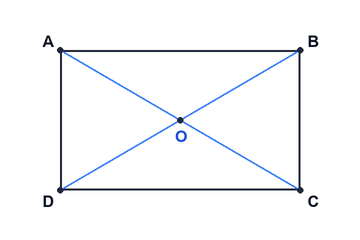
\includegraphics[width=\linewidth]{images/de1_cau11.png}
	\end{minipage}
	\loigiai{
		Trong hình chữ nhật, hai đường chéo bằng nhau. Do đó khẳng định đúng là $AC = BD$.
	}
\end{ex}

\begin{ex}%Câu 12
	\noindent
	\begin{minipage}[t]{0.70\linewidth}
		Hình thoi $MNPQ$ ở hình bên có hai đường chéo $MP = 8\text{ cm}$, $NQ = 6\text{ cm}$. Diện tích hình thoi $MNPQ$ là
		\choice
		{$48\text{ cm}^2$}
		{$14\text{ cm}^2$}
		{$28\text{ cm}^2$}
		{\True $24\text{ cm}^2$}
	\end{minipage}\hfill
	\begin{minipage}[t]{0.26\linewidth}
		\centering\vspace{0pt}
		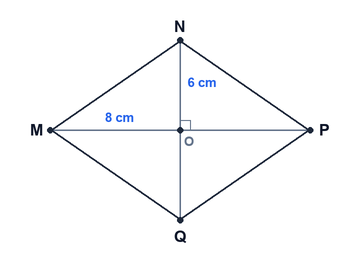
\includegraphics[width=\linewidth]{images/de1_cau12.png}
	\end{minipage}
	\loigiai{
		Diện tích hình thoi bằng nửa tích độ dài hai đường chéo:
		\[ S = \frac{1}{2} \cdot 8 \cdot 6 = 24\text{ (cm}^2\text{)}. \]
	}
\end{ex}

\vspace{8pt}

% ------------------------------------------------------------------------------
% PHẦN II: CÂU TRẮC NGHIỆM ĐÚNG SAI
% ------------------------------------------------------------------------------
\noindent\textbf{PHẦN II. Câu trắc nghiệm đúng sai (2,0 điểm).}\\
\textit{Thí sinh trả lời từ câu 13 đến câu 14. Trong mỗi ý a), b), c), d) ở mỗi câu, thí sinh chọn đúng hoặc sai.}

\begin{ex}%Câu 13
	Cho hai số $a = 72$ và $b = 108$.
	\choiceTF
	{\True $a$ chia hết cho $9$}
	{$b$ là số nguyên tố}
	{\True $\text{ƯCLN}(a, b) = 36$}
	{Có đúng $4$ bội chung khác $0$ của $a$ và $b$ nhỏ hơn $700$}
	\loigiai{
		\begin{itemchoice}
			\item Đúng: $7 + 2 = 9$ chia hết cho $9$ nên $72 \ \vdots \ 9$.
			\item Sai: $108$ có chữ số tận cùng là $8$ nên chia hết cho $2$ (có các ước khác $1$ và chính nó), do đó $b$ là hợp số.
			\item Đúng: Phân tích ra thừa số nguyên tố: $72 = 2^3 \cdot 3^2$ và $108 = 2^2 \cdot 3^3$. Suy ra $\text{ƯCLN}(a, b) = 2^2 \cdot 3^2 = 36$.
			\item Sai: $\text{BCNN}(a, b) = 2^3 \cdot 3^3 = 216$. Các bội chung khác $0$ của $a$ và $b$ nhỏ hơn $700$ là: $216; 432; 648$, chỉ có $3$ số.
		\end{itemchoice}
	}
\end{ex}

\begin{ex}%Câu 14
	\noindent
	\begin{minipage}[t]{0.68\linewidth}
		Một mảnh bìa hình chữ nhật $ABCD$ có $AB = 10\text{ cm}$, $BC = 6\text{ cm}$. Trên cạnh $AB$ lấy điểm $E$, trên cạnh $CD$ lấy điểm $F$ sao cho $AE = DF = 4\text{ cm}$ (hình bên).
		\choiceTF
		{\True $CD = 10\text{ cm}$}
		{Hình chữ nhật $ABCD$ có hai đường chéo vuông góc với nhau}
		{\True Diện tích tứ giác $EBCF$ bằng $36\text{ cm}^2$}
		{\True Cắt mảnh bìa theo đoạn thẳng $EF$ được hai mảnh. Tổng chu vi hai mảnh lớn hơn chu vi mảnh bìa ban đầu là $12\text{ cm}$}
	\end{minipage}\hfill
	\begin{minipage}[t]{0.28\linewidth}
		\centering\vspace{0pt}
		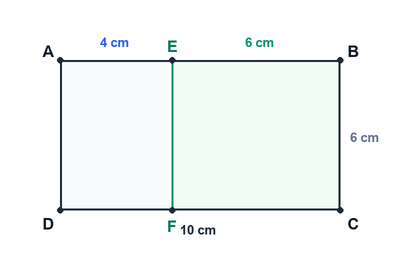
\includegraphics[width=\linewidth]{images/de1_cau14.png}
	\end{minipage}
	\loigiai{
		\begin{itemchoice}
			\item Đúng: Trong hình chữ nhật, các cạnh đối bằng nhau nên $CD = AB = 10\text{ cm}$.
			\item Sai: Hình chữ nhật có hai đường chéo bằng nhau; vì $AB \neq BC$ nên hai đường chéo không vuông góc với nhau.
			\item Đúng: Ta có $EB = AB - AE = 10 - 4 = 6\text{ cm}$ và $FC = CD - DF = 10 - 4 = 6\text{ cm}$. Tứ giác $EBCF$ là hình vuông cạnh $6\text{ cm}$ nên có diện tích $6 \cdot 6 = 36\text{ cm}^2$.
			\item Đúng: Chu vi hình chữ nhật $AEFD$ là $(4 + 6) \cdot 2 = 20\text{ cm}$; chu vi hình vuông $EBCF$ là $4 \cdot 6 = 24\text{ cm}$. Chu vi hình chữ nhật ban đầu $ABCD$ là $(10 + 6) \cdot 2 = 32\text{ cm}$. Tổng chu vi hai mảnh lớn hơn chu vi ban đầu là: $20 + 24 - 32 = 12\text{ cm}$ (chính bằng $2 \cdot EF = 2 \cdot 6 = 12\text{ cm}$).
		\end{itemchoice}
	}
\end{ex}

\vspace{8pt}

% ------------------------------------------------------------------------------
% PHẦN III: CÂU TRẮC NGHIỆM TRẢ LỜI NGẮN
% ------------------------------------------------------------------------------
\noindent\textbf{PHẦN III. Câu trắc nghiệm trả lời ngắn (2,0 điểm).}\\
\textit{Thí sinh trả lời từ câu 15 đến câu 18.}

\begin{ex}%Câu 15
	Tính giá trị của biểu thức $2^5 - 5^2$.
	\shortans{7}
	\loigiai{
		$2^5 - 5^2 = 32 - 25 = 7$.
	}
\end{ex}

\begin{ex}%Câu 16
	Tìm chữ số $x$ để số $\overline{25x}$ chia hết cho cả $3$ và $5$.
	\shortans{5}
	\loigiai{
		Vì $\overline{25x}$ chia hết cho $5$ nên $x \in \{0; 5\}$.
		\begin{itemize}
			\item Với $x = 0$, tổng các chữ số là $2 + 5 + 0 = 7$ không chia hết cho $3$.
			\item Với $x = 5$, tổng các chữ số là $2 + 5 + 5 = 12$ chia hết cho $3$.
		\end{itemize}
		Vậy chữ số cần tìm là $x = 5$.
	}
\end{ex}

\begin{ex}%Câu 17
	\noindent
	\begin{minipage}[t]{0.70\linewidth}
		Hình bình hành $ABCD$ ở hình bên có cạnh $CD = 9\text{ cm}$, chiều cao $AH = 5\text{ cm}$. Tính diện tích hình bình hành $ABCD$ (đơn vị: $\text{cm}^2$).
		\shortans{45}
	\end{minipage}\hfill
	\begin{minipage}[t]{0.26\linewidth}
		\centering\vspace{0pt}
		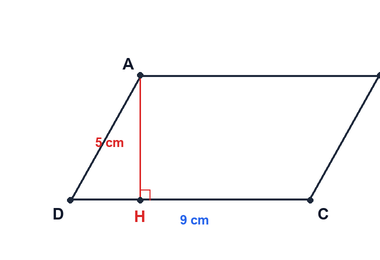
\includegraphics[width=\linewidth]{images/de1_cau17.png}
	\end{minipage}
	\loigiai{
		Diện tích hình bình hành $ABCD$ là:
		\[ S = CD \cdot AH = 9 \cdot 5 = 45\text{ (cm}^2\text{)}. \]
	}
\end{ex}

\begin{ex}%Câu 18
	Bạn Minh mua $5$ quyển vở, giá $12\,000$ đồng một quyển và $3$ chiếc bút bi, giá $8\,000$ đồng một chiếc. Minh đưa cho người bán tờ $100\,000$ đồng. Hỏi người bán phải trả lại Minh bao nhiêu nghìn đồng?
	\shortans{16}
	\loigiai{
		Tổng số tiền Minh phải trả là:
		\[ 5 \cdot 12\,000 + 3 \cdot 8\,000 = 60\,000 + 24\,000 = 84\,000\text{ (đồng)}. \]
		Số tiền người bán phải trả lại cho Minh là:
		\[ 100\,000 - 84\,000 = 16\,000\text{ (đồng)}, \]
		tức là $16$ nghìn đồng.
	}
\end{ex}


